\section{RESULTS}
\label{sec:results}

All the modules described in the previous section were
conveniently integrated in workflows using \emph{nipype}
\cite{gorgolewski_nipype:_2011}. The choice of this tool
grants the reproducibility of the experiments,
and the evaluation workflow is publicly released.
The results of the proposed experiments are summarized
in \autoref{fig:results} and \autoref{table:results}.
The remaining of this section provides extended descriptions
and interpretation of the results.

\begin{figure*}[tpb]
   \centering
   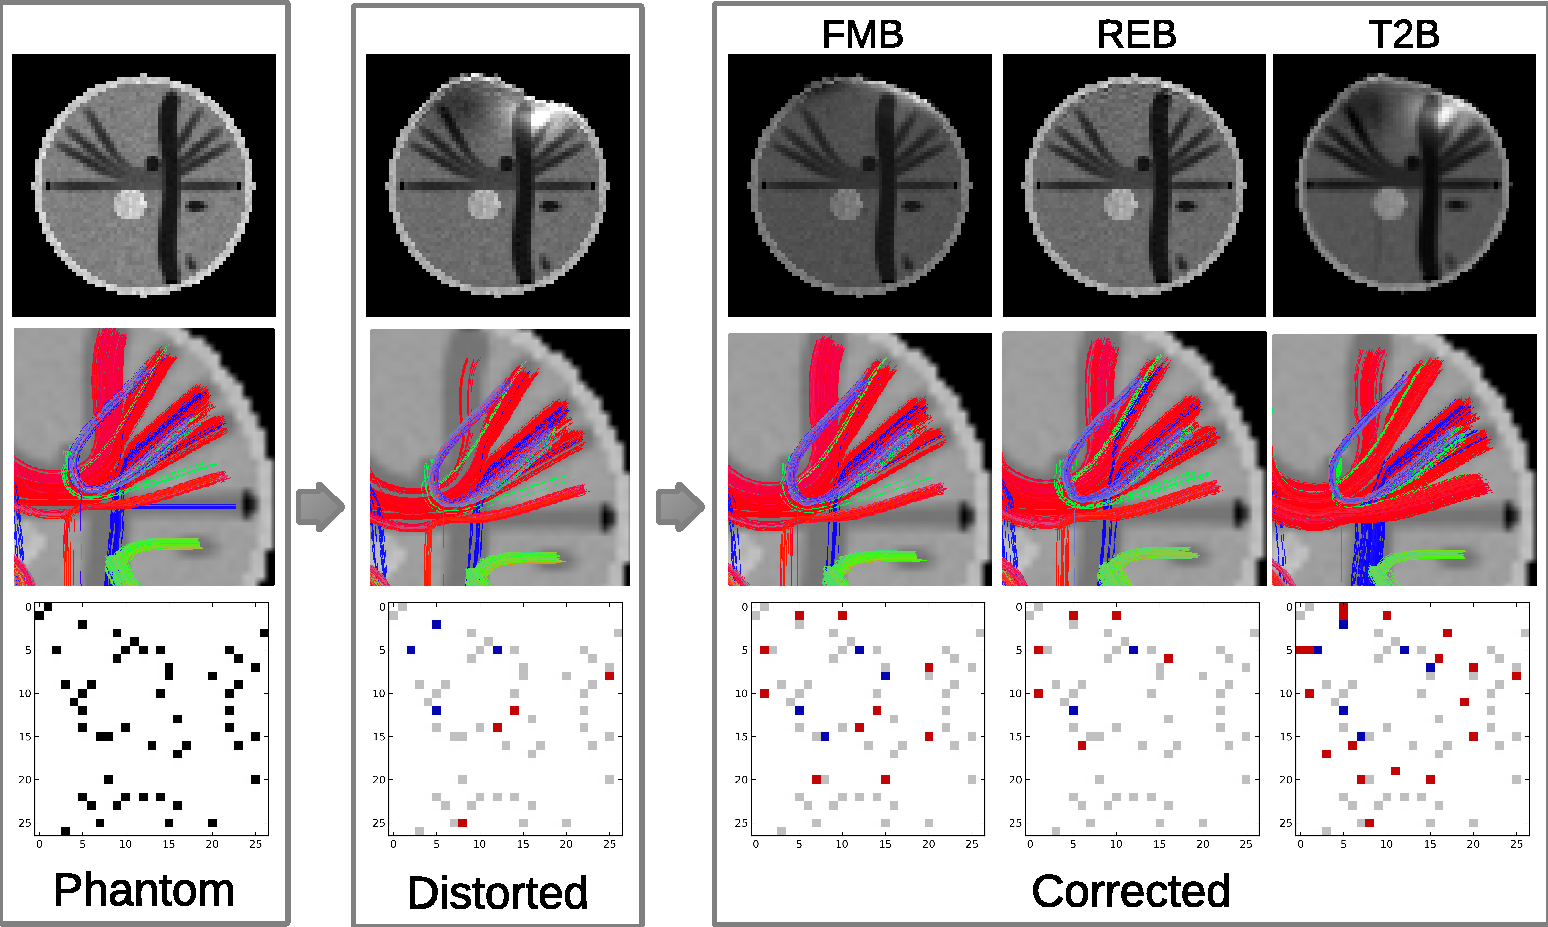
\includegraphics[width=0.9\textwidth]{Fig02-Results}
   \caption{Visual evaluation of the correction methods.
   First row represents a coronal section of the \textit{b0} volume. 
   In second row, the outcome of tractography after filtering tracks
   that did not connect two regions.
   Third row shows the associated connectivity matrices. All the matrices
   are compared to the ground-truth connections in the phantom. The existing
   connections that were correctly detected at each step are depicted in white
   color. False positives have been marked in red and false negatives in blue.
   Gray color represents the true negatives (non-existent connections correctly detected).}
   \label{fig:results}
\end{figure*}


\subsection{Geometrical correctness and signal recovery}

A summary of quantitative results, computed for the \gls*{dti} 
dataset with maximum shift of 3.80~mm,
is provided in \autoref{table:results}.
The best scores were obtained with the \gls*{reb} 
method, followed by \gls*{fmb}. 
The clear difference of accuracy between \gls*{reb} and \gls*{fmb}
with respect to \gls*{t2b} infers the latter may not be
an appropriate method for susceptibility correction. 
The described performance was constant for \gls*{fmb} 
and \gls*{reb} along the different magnitudes of 
distortion evaluated (maximum phase-encoding direction 
shifts in the range of 3.80-7.60~mm).


\begin{table}[!t]
\caption{Accuracy results}
\label{table:results}
\begin{center}
\begin{tabular}{c||cccc|cc}
\hline
 & \multicolumn{4}{c|}{ Overlap (Jaccard Index, \%)} & \multicolumn{2}{c}{ Signal Correlation (\%)} \\
\hline
 & Av. & \gls*{csf} & \gls*{wm} & \gls*{gm} & \textit{b0} & \glspl*{dwi} \\
\hline
\gls*{fmb} & $93.00$ & $88.57$ & $96.74$ & $94.02$ & $80.05$ & $96.26\pm.06$ \\
\hline
\gls*{reb} & $96.64$ & $94.31$ & $98.26$ & $96.75$ & $91.00$ & $97.65\pm.03$ \\
\hline
\gls*{t2b} & $79.19$ & $66.31$ & $89.85$ & $82.14$ & $64.58$ & $90.10\pm.13$ \\
\hline
\end{tabular}
\end{center}
\end{table}

A second workflow investigated the similarity of the recovered
signal with respect to the original (undistorted).
In this second study, \gls*{reb} performed
better than the other two methods, as reported
in \autoref{table:results}. \gls*{reb} scored a $91.0\%$
similarity index for the \textit{b0} volume and an average $97.65\%$
for the remaining \glspl*{dwi}. Again, the second
qualified was \gls*{fmb}, which achieved very close results
for the \glspl*{dwi} ($96.26\%$) but not as good for the \textit{b0}
volume. Visual inspection of the recovered data confirms the 
presented quantitative results (\autoref{fig:results}, first row).


\begin{table}[!t]
\caption{Tractography and connectivity results.}
\label{table:results-tractography}
\footnotesize
\begin{center}
\begin{tabular}{l||cccc}
\hline
 & \# tracks & length (mm) & FP & FN \\
\hline
Original & 735 & $40.87\pm13.55$ & 40 & 4 \\
\hline
Distorted & 878 & $40.54\pm13.73$ & 42 & 4 \\
\hline
\gls*{fmb} & 743 & $40.04\pm13.60$ & 43 & 4 \\
\hline
\gls*{reb} & 830 & $39.87\pm13.93$ & 44 & 4 \\
\hline
\gls*{t2b} & 825 & $41.44\pm12.85$ & 40 & 5 \\
\hline
\end{tabular}
\end{center}
\end{table}

\subsection{Impact on tractography and connectivity}

Connectivity matrices derived from the \gls*{dti} dataset
were completely hindered by the high complexity of the 
fibers contained
in the phantom. Tractography discovered successfully only 4 out 
of 27 existing connections from the original (undistorted) data,
with more than 45 false connections.
With the \gls*{hardi} dataset (reconstructed with constrained 
spherical deconvolution) we found 23/27 connections,
but we still observed 40 false positives. Therefore, the 
experiments using the \gls*{dti} phantom were discarded. The
results presented in this subsection only refer to the 
\gls*{hardi} dataset.

Using the strongest distortion (maximum shift of 7.60~mm),
the number of detected connections
remained the same (23/27), slightly increasing the number of
false positives to 42. The immediate conclusion is that, with highly
complex anatomies (crossing, fanning, etc.) and limited number of
ground-truth connections, connectivity matrices are more sensitive 
to reconstruction and tractography than to distortions.

For the sake of completeness, \autoref{table:results-tractography}
reports the characteristic features of the tractography results
and connectivity matrices, for the fieldmap that caused a maximum
shift of 3.80~mm. Very similar results were obtained for
7.60~mm. This results, along with visual inspection
(\autoref{fig:results}, second and third rows), might point
to \gls*{fmb} as the best correction method.


\subsection{Discussion}

Even though all the surveyed methods produced visually 
sound results, our study suggested that \gls*{reb} is the 
most accurate method in terms of geometrical accuracy and
signal dropout recovery. 
The \gls*{t2b} method did not achieve the necessary high-standards
to recommend its use. Nonetheless, we understand that specific
methods with anisotropic regularization that completely
restrict deformations to the phase-encoding direction would perform
significantly better than the standard method presented.
Geometrical correctness of \gls*{dwi} data is fundamental 
in connectivity analysis to spatially locate the
regions which will define the nodes of the final connectivity
matrix.

Regarding tractography, this study revealed that signal
reconstruction and tractography algorithms masked the 
impact of susceptibility distortion on the final connectivity
matrices. Due to this effect, experiments performed on 
the \gls*{dti} phantom were discarded for comparison.
With the \gls*{hardi} dataset, the extracted 
connectivity matrix slightly
changed with distortion. Quantitative differences reported in
\autoref{table:results-tractography} could be more related
to the smoothing derived from interpolation implemented by
each method. Visual results might suggest that \gls*{fmb}
achieved better results.

Although we found connectivity matrices rather invariant with
respect distortion, they are suspected to be significantly
impacted by the susceptibility artifact on real data 
\cite{irfanoglu_effects_2012}.
This hypothesis points to the need of more appropriate 
phantoms with denser connectivity matrices.
State of the art phantoms for tractography usually present a
discrete set of simulated fiber bundles that translate in 
very sparse fiber-endings regions and connectivity matrix.
In the real case, the surface limiting the tracks is densely 
covered by the regions mapped from the anatomical 
dataset, what leads to larger sensitivity with respect 
deformations.

A possible limitation of this work is that \gls*{fmb} is
used for both synthesis and correction of the distortion.
However, practical reasons (i.e. noise, signal dropout)
impede perfect geometrical correction with \gls*{fmb}.
Moreover, \gls*{reb} performed more accurately 
than \gls*{fmb}.

Future extensions of this work will include a 
refined digital phantom. Additional lines for this
work will evaluate different realizations of the 
synthetic phase-difference map, to better characterize
the phenomenon. Also, the framework can be enhanced 
for studying the impact of other artifacts as 
subject's motion or eddy currents-derived distortions.